\chapter{Design Pattern}
\section{Design Pattern, cosa sono?}
I \textbf{Design Pattern} sono \textit{soluzioni progettuali generali a problemi ricorrenti}. Si tratta di una descrizione o modello logico da applicare per risolvere un problema, il quale può presentarsi in diverse situazioni durante le fasi di progettazione e sviluppo del software.\\
Vanno definiti prima della codifica, questo permette di contenere e ridurre i problemi futuri dello sviluppo di un software.\\
I design pattern tipicamente mostrano relazioni ed interazioni tra \textit{classi} o \textit{oggetti}, senza specificare le classi applicative finali coinvolte.

\subsection{Come sono costituiti}
Un \textit{design pattern} è costituito da:
\begin{itemize}
	\item \textit{il nome}, costituito da una o più parole che siano rappresentative del pattern stesso;
	\item \textit{il problema}, ovvero la descrizione della situazione alla quale si può applicare il pattern. Può comprendere la descrizione di classi o di problemi di progettazione specifici, come anche una lista di condizioni perchè sia necessario l'utilizzo del pattern
	\item \textit{la soluzione}, che descrive gli elementi che costituiscono il progetto, le relazioni e le relative implicazioni, senza addentrarsi in una specifica implementazione. In poche parole bisogna rappresentare un problema astratto e la relativa configurazione di elementi adatta a risolverlo.
	\item \textit{le conseguenze}, risultati e vincoli che derivano dall'applicazione del pattern. Le conseguenze comprendono considerazioni di tempo e di spazio, possono descrivere implicazioni del pattern con alcuni linguaggi di programmazione e l'impatto con il resto del progetto. Sono fondamentali in quanto aiutano nella scelta dei pattern.
\end{itemize}
I design pattern possono essere classificati in tre principali categorie, che risolvono problemi diversi. Questi tipi di pattern sono di tipo \textit{Strutturale, Creazionale e Comportamentale}, e verranno approfonditi nei prossimi paragrafi.

\section{Design Pattern Strutturali}
I \textit{design pattern strutturali} sono relativi a come classi ed oggetti sono composti per formare strutture più complesse. In generale possiamo distinguere due tipologie di pattern strutturali:
\begin{itemize}
\item basati su \textbf{classi}, i quali utilizzano l'ereditarietà per generare classi che combinano le proprietà di classi base.
\item basati su \textbf{oggetti}, i quali mostrano come comporre gli oggetti al fine di estendere, in fase di esecuzione, le funzionalità di una classe (cosa non possibile nel caso della composizione statica tramite ereditarietà).
\end{itemize}
La maggior parte dei pattern strutturali sono basati sugli oggetti.
Di seguito andremo ad analizzare i principali pattern strutturali conosciuti.
\subsection{Adapter}
\subsubsection{Cos'è?}
Adapter, chiamato anche \textit{wrapper}, è un design pattern strutturale che può essere basato sia su \textit{classi} che su \textit{oggetti}.\\
Il suo obiettivo è fornire una soluzione al problema dell'interoperabilità tra interfacce differenti.
\subsubsection{Applicabilità}
L'uso di questo pattern risulta utile quando interfacce di classi differenti devono poter comunicare tra loro, oppure quando si desidera che l'invocazione di un metodo di un oggetto da parte dei client avvenga in maniera "indiretta", ovvero che invece di richiamare il metodo direttamente, si passi attraverso dei metodi "pubblici" che fanno da tramite con l'esterno. Questo permette alla classe di subire motifiche future mantenendo la retrocompatibilità.

\subsubsection{Composizione}
Adapter può essere basato su classi, utilizzando l'ereditarietà multipla per adattare interfacce diverse con il meccanismo dell'ereditarietà, oppure sulla composizione di oggetti.\\
I partecipanti del pattern sono:
\begin{itemize}
	\item Adaptee: definisce l'interfaccia che necessità di essere adattata;
	\item Target: definisce l'interfaccia che usa il Client;
	\item Client: collabora con gli oggetti in conformità con l'interfaccia Target;
	\item Adapter: adatta l'interfaccia Adaptee all'interfaccia Target.
\end{itemize}

\begin{figure}[H]
	\centering
	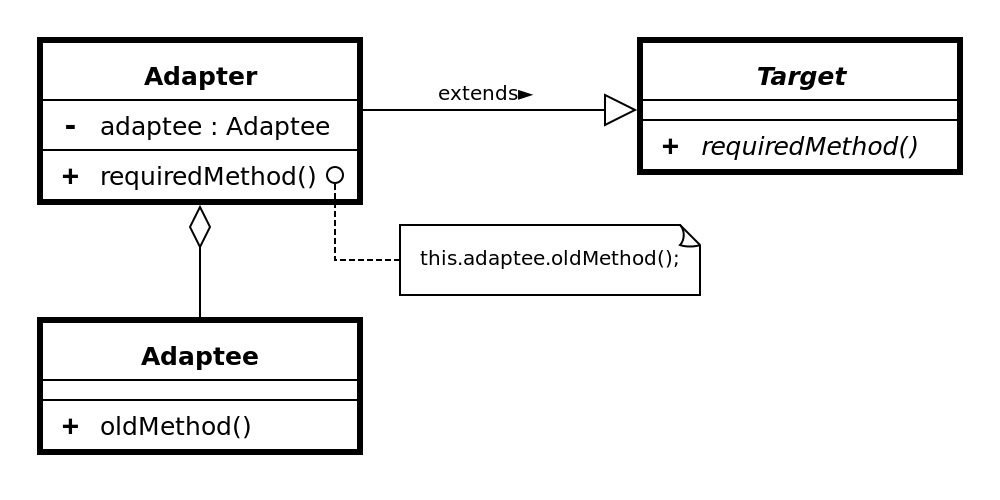
\includegraphics[width=0.7\linewidth]{res/img/DP_Adapter}
	\caption{Diagramma UML del Pattern Adapter}
	\label{fig:dpadapter}
\end{figure}

\subsection{Bridge}
\subsection{Composite}
\subsection{Container}
\subsection{Decorator}
\subsection{Façade}
\subsection{Proxy}
\subsection{Flyweight}

\section{Design Pattern Creazionali}

\section{Design Pattern Comportamentali}

